\documentclass[fleqn]{article}
\oddsidemargin 0.0in
\textwidth 6.0in
\thispagestyle{empty}
\usepackage{import}
\usepackage{amsmath}
\usepackage{graphicx}
\usepackage{flexisym}
\usepackage{calligra}
\usepackage{amssymb}
\usepackage{bigints} 
\usepackage[english]{babel}
\usepackage[utf8x]{inputenc}
\usepackage{float}
\usepackage[colorinlistoftodos]{todonotes}


\DeclareMathAlphabet{\mathcalligra}{T1}{calligra}{m}{n}
\DeclareFontShape{T1}{calligra}{m}{n}{<->s*[2.2]callig15}{}
\newcommand{\scriptr}{\mathcalligra{r}\,}
\newcommand{\boldscriptr}{\pmb{\mathcalligra{r}}\,}

\definecolor{hwColor}{HTML}{442020}

\begin{document}

  \begin{titlepage}

    \newcommand{\HRule}{\rule{\linewidth}{0.5mm}}

    \center

    \begin{center}
      
\includegraphics[height=11cm, width=11cm]{asu.png}
    \end{center}

    \vline

    \textsc{\LARGE Statistical/Thermal Physics}\\[1.5cm]

    \HRule \\[0.5cm]
    { \huge \bfseries Homework 6}\\[0.4cm] 
    \HRule \\[1.0cm]

    \textbf{Behnam Amiri}

    \bigbreak

    \textbf{Prof: Michael Treacy}

    \bigbreak

    \textbf{{\large \today}\\[2cm]}

    \vfill

  \end{titlepage}

  \begin{enumerate}
    \item \textbf{3.1} Use Table 3.1 to compute the temperature of solid A and solid B when $q_A=1$. Then
    compute both temperatures when $q_A=60$. Express your answers in terms of $\epsilon/k$ and then in 
    kelvins assuming that $\epsilon=0.1 ~ eV$.

      \begin{center}
        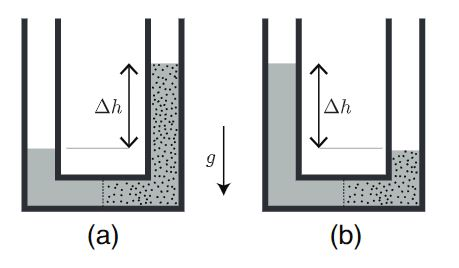
\includegraphics[height=10cm, width=14cm]{1.JPG}
      \end{center}

    \pagebreak

    \item \textbf{3.5} Starting with the result of problem 2.17, find a formula for the temperature of an Einstein 
    solid in the limit $q << N$. Solve for the energy as a function of temperature to obtain 
    $U=N \epsilon e^{-\epsilon/k T}$ (where $\epsilon$ is the size of an energy unit).

      \begin{center}
        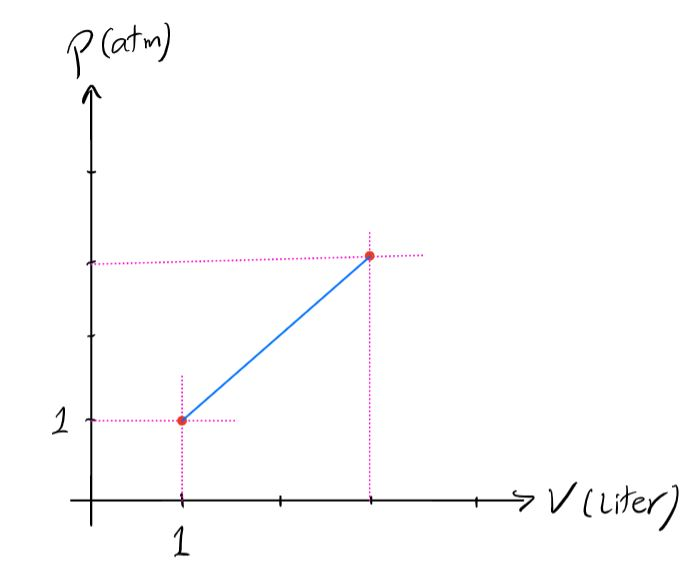
\includegraphics[height=10cm, width=14cm]{2.JPG}
      \end{center}

    \pagebreak

    \item \textbf{3.7} Use the result of Problem 2.42 to calculate the temperature of a black hole, in terms
    of its mass $M$. (The enrgy is $Mc^2$.) Evaluate the resulting expression for a one-solar-mass black hole.
    Also sketch the entrophy as a function of energy, and discuss the implications of the shape of the graph. 

      \begin{center}
        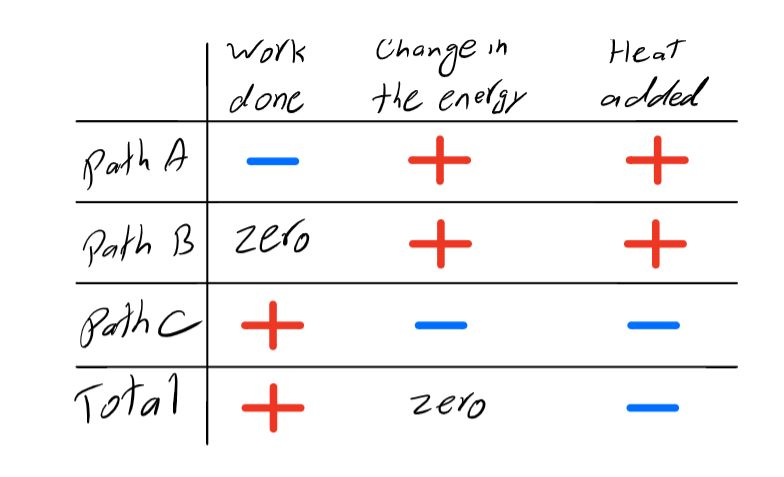
\includegraphics[height=10cm, width=14cm]{3.JPG}
      \end{center}

    \pagebreak

    \item \textbf{3.9} In solid carbon monoxide, each CO molecule has two possible orientations: CO or 
    OC. Assuming that these orientations are completely random (not quite true but close), calculate
    the residual entrophy of a mole of carbon monoxide.

      \begin{center}
        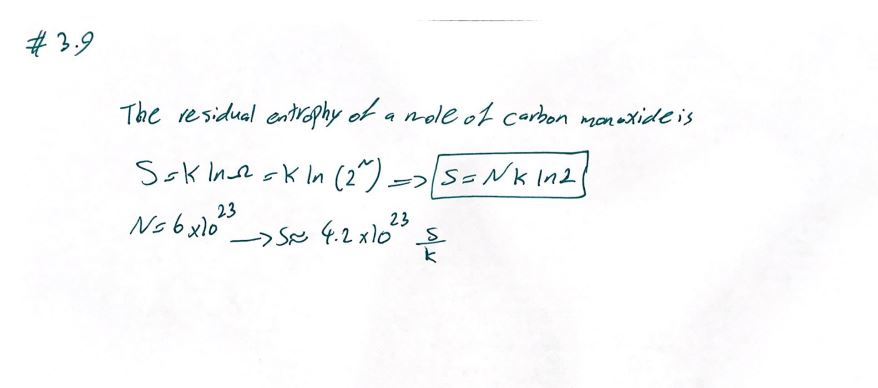
\includegraphics[height=10cm, width=14cm]{4.JPG}
      \end{center}

    \pagebreak

    \item \textbf{3.10} An ice cube (mass $30 ~ g$) at $0^{\circ} ~ C$ is left sitting on the kitchen table,
    where it gradually melts. The temperature in the kitchen is $25^{\circ} ~ C$

      \begin{center}
        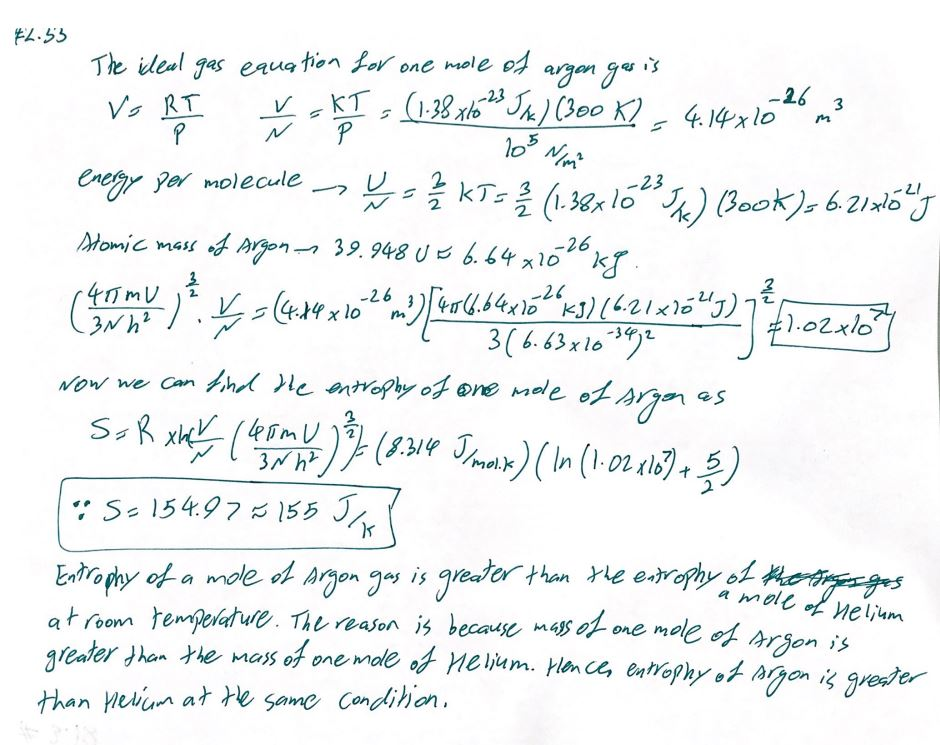
\includegraphics[height=10cm, width=14cm]{5.JPG}
      \end{center}

    \pagebreak

    \item \textbf{3.14} Experimental measurements of the heat capacity of aluminum at low temperatures 
    (below about $50 ~ K$) can be fit to the formula
    $$
      C_V=aT+bT^3,
    $$ where $C_V$ is the heat capacity of one mole...

      \begin{center}
        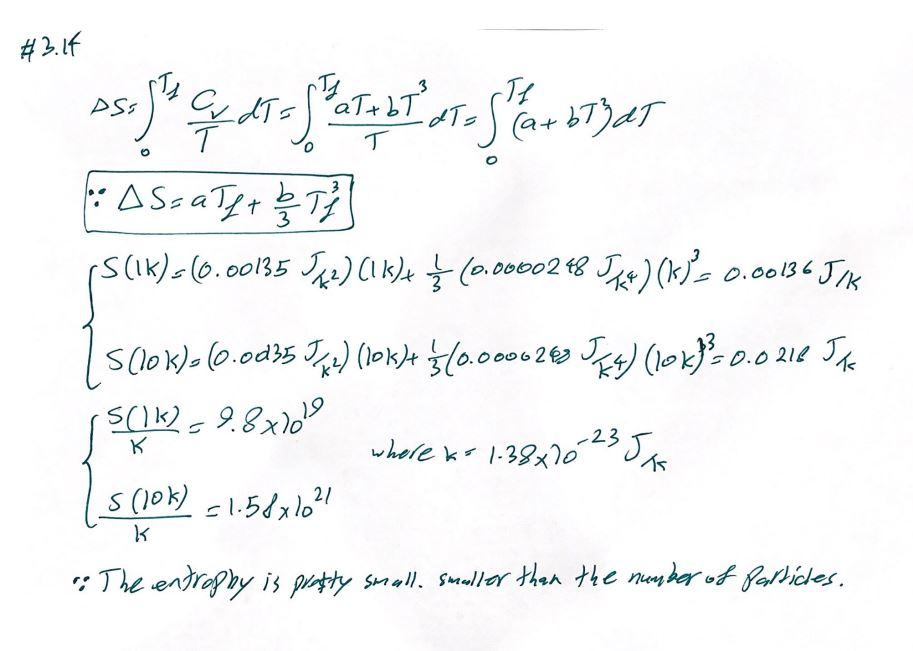
\includegraphics[height=10cm, width=14cm]{6.JPG}
      \end{center}

    \pagebreak

    \item \textbf{3.18} Use a computer to reproduce Table 3.2 and the associated graphs of energy, temperature,
    heat capacity, and magnetization. (The graphs in this section are actually drawn from the analytic formulas
    derived below, so your numerical graphs won't be quite smooth.)

      % \textcolor{hwColor}{
      %   \\
      % }

  \end{enumerate}

\end{document}
